\chapter{绪论}

\section{课题背景与意义}

实时绘制(real-time rendering)是计算机图形学(computer graphics)领域中对交互性要求最高的一项技术,其中“实时”(real-time)二字意味着这样一个循环往复的过程:屏幕上更新了一帧新的图像,用户观察到新的图像并作出反馈,这些反馈又影响下一帧图像的内容。在计算机图形学领域,我们往往用每秒生成的图像个数(frames per second),简称帧率,来衡量图像生成的速度。为了实现良好的交互体验,帧率必须要达到较高的水平。反之,如果图像不能及时地随着用户输入而更新,将破坏用户的沉浸感。实时绘制技术即是追求计算机图像的快速生成的一项技术。当然,在追求图像生成速度的同时,实时绘制技术也将图像的质量考虑在内,要在保证帧率满足要求的条件下尽可能实现高质量的图像。

\begin{figure}[!t]
    \centering
    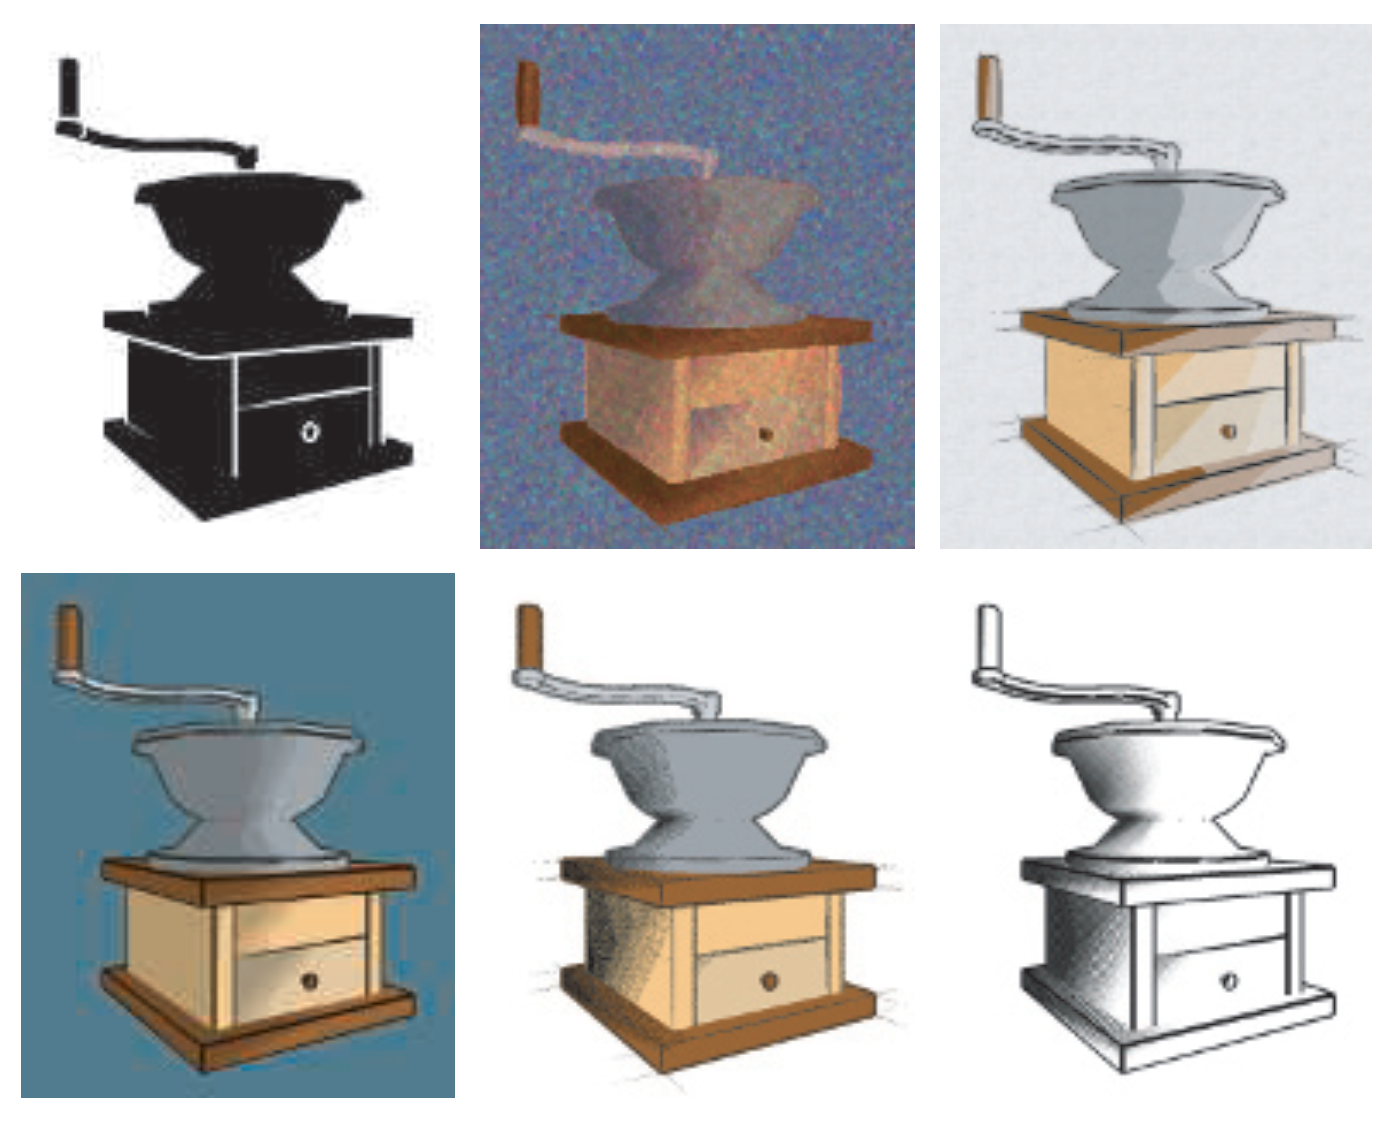
\includegraphics[width=\linewidth]{npr}
    \caption{\label{fig:npr}
    使用不同的艺术风格对一个咖啡机模型进行非真实感绘制}
\end{figure}

\begin{figure}[!b]
    \centering
    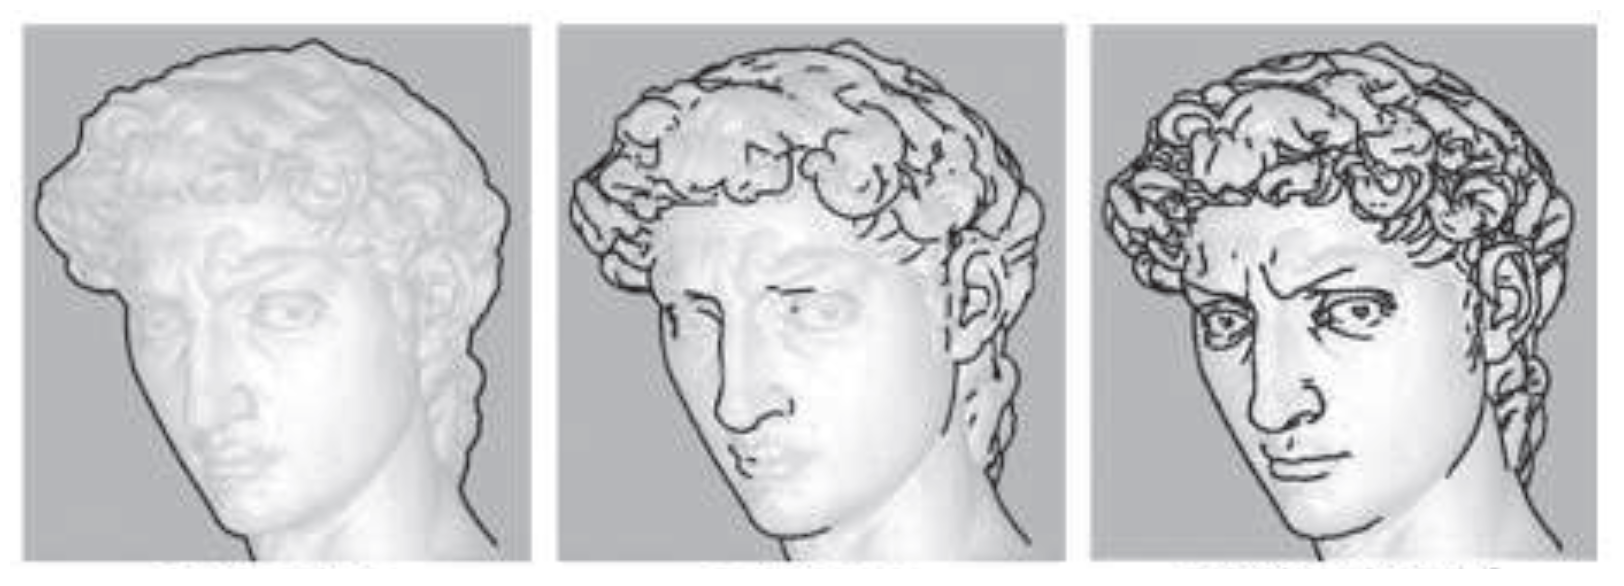
\includegraphics[width=\linewidth]{npr_lines}
    \caption{\label{fig:npr_lines}
    从左到右:外轮廓线,\con{},以及\con{}加上\scon{}的结果}
\end{figure}

就图像表现而言,实时绘制技术可以分为真实感绘制(photorealistic rendering)和\npr{}(non-photorealistic rendering)两个不同的方向。真实感绘制追求与现实世界一致的图像表现,使得用户在计算机生成的虚拟图像上体会到真实感。与之相反,\npr{}技术生成的图像与现实世界相差甚远。\npr{}旨在表现特定的卡通或简约的艺术风格,因而又称为风格化绘制(stylized rendering),来自\cite{akenine2018real}的\autoref{fig:npr}展示了一个对三维模型进行不同风格的非真实感绘制的例子。具体而言,\npr{}主要包含两个方面的技术:风格化着色(stylized shading)和线绘制(line rendering)。风格化着色旨在通过设计着色方式来表现特定的艺术风格,例如卡通着色和铅笔画风格着色。而线绘制旨在通过绘制线条来达到强调物体轮廓或简化物体外表的效果,该技术往往和不同的风格化着色搭配使用,是\npr{}中最为常用也是研究最多的一项技术。线绘制包含对各式各样的线条进行绘制的技术,例如外轮廓线(silhouette),\con{}(contour),以及\scon{}(suggestive contour)。来自\cite{akenine2018real}的\autoref{fig:npr_lines}展示了这三种线绘制技术中讨论较多的线条。本文将针对线绘制中的\con{}绘制和\scon{}绘制进行探讨。出于行文简洁的考虑,下文将三维模型表面上组成\con{}和\scon{}的点称为轮廓点,同样地,将组成\vdl{}的点成为\vdp{}。

\begin{figure}[!t]
    \centering
    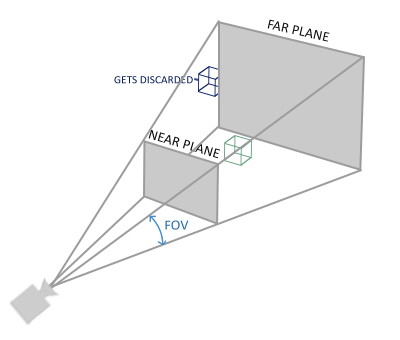
\includegraphics[width=0.6\linewidth]{view}
    \caption{\label{fig:view}
    视锥体}
\end{figure}

\begin{figure}[!b]
    \centering
    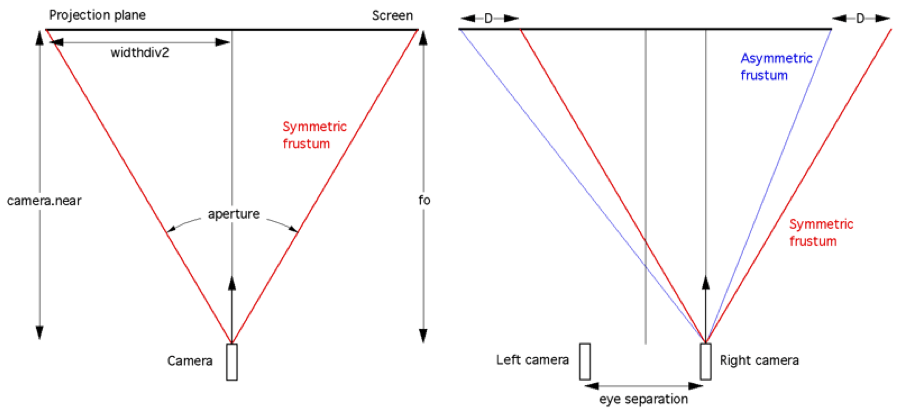
\includegraphics[width=\linewidth]{stereo}
    \caption{\label{fig:stereo}
    单目绘制和双目绘制的区别}
\end{figure}

就交互形式而言,实时绘制技术又可以分为单目绘制(monoscopic rendering)和双目绘制(stereoscopic rendering),二者的区别在于视点(viewpoint)的数目。视点是图形绘制系统中很重要的构成部分,它和光源、场景一起决定了最终绘制得到的画面。视点定义了绘制所得画面的观察位置和角度。具体而言,每个视点对应了一个视锥体(view frustum),绘制场景中只有位于视锥体内的物体部分会参与绘制并影响最终得到的画面。来自\cite{learnopengl}的\autoref{fig:view}中展示了常见的视锥体的结构。
一般而言,图形程序只需要绘制单个视点所观察的图像,即单目绘制。而对于虚拟现实这类旨在提供三维立体感的应用,则需要绘制两个对应于双眼的视点所观察的图像从而模拟立体视觉,即双目绘制。来自\cite{topicsinopengl}的\autoref{fig:stereo}展示了单目绘制和双目绘制在视点以及视锥体上的区别。显然,由于需要对两个不同的视点进行绘制,双目绘制所需要的计算量相比于单目绘制更高,实现实时的双目绘制比起一般的实时绘制更有挑战性。尽管GPU的计算性能随着硬件技术的发展而逐年提升,但实现实时的双目绘制仍然并非易事。再者,双目绘制对于图像的质量有着更高的要求。就\vdl{}的双目绘制而言,如果只是直接地分别以两眼为视点分别进行绘制,绘制得到的轮廓线将不满足立体一致。而如果不能满足立体一致的要求,将会严重影响用户的体验甚至造成用户不适。因此,如何快速并正确地对\vdp{}进行双目绘制,是一个非常有研究价值的问题。

\begin{figure}[!t]
    \centering
    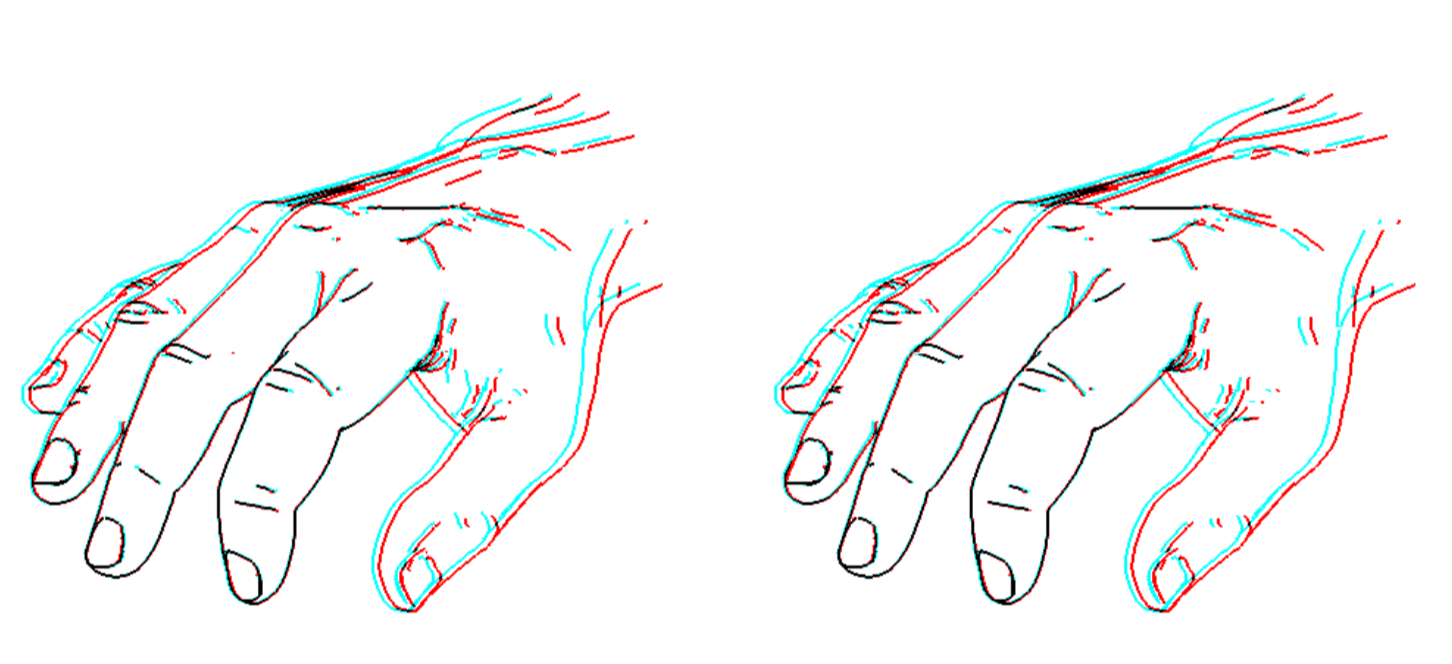
\includegraphics[width=\linewidth]{hands}
    \caption{\label{fig:hands}
    左:直接对两眼分别进行绘制,右:立体一致的轮廓线}
\end{figure}

\citeauthor{kim2013stereoscopic}在此前提出了一个\stc{}线绘制方法\cite{kim2013stereoscopic},该方法通过消除那些在另一个视点中没有对应点的\vdp{}来保证立体一致性,\autoref{fig:hands}是他们的文章中给出的对比结果。该方法的核心在于:采样多个两眼之间的视点位置绘制出多张图像,接着判定\vdp{}在这些图像中的连续性。该方法能够实现\stc{}\vdl{}绘制,但是对于复杂的物体表面而言,需要采样大量的视点来减少匹配的错误。因此,该方法需要较长的计算时间,不适用于实时绘制类型的应用。

\section{研究内容与贡献}

本文提出了一种对\stc{}\vdl{}进行实时绘制的方法。在\citeauthor{kim2013stereoscopic}的工作的基础上,本文设计了一种图像空间的搜索算法来验证\vdp{}的\epsl{}(epipolar-slidability)。本文方法的出发点在于:对于每个位于对极曲线(epipolar-curve)上的表面点,有一个对应的位于两眼连线上的一个视点将该表面点视为\conp{}(或\sconp{})。在此出发点的基础上,我们可以将\epsl{}的判定转换为检查这些\vdp{}的对应视点的轨迹。当这些轨迹是单调地从左眼移动到右眼,或者单调地从右眼移动到左眼,那么其对应的\vdp{}是对极可滑动(epipolar-slidable)的。接着,只需要去检查这些轨迹上的极值点便可判定其单调性。这个过程可以在图像空间中一次过完成,而不需要像之前的方法一样对多个视点进行采样,因而节省了大量的计算时间。这个检查对应视点的轨迹的想法对\con{}和\scon{}都适用,只是对于\scon{}而言,除了轨迹的极值点之外还需要检查轨迹的区间端点。另外,为了避免因为\conp{}或\sconp{}的重叠而导致的匹配错误,本文设计的方法使用了GPU上的\ppll{}\cite{yang2010real}来保存位于同一像素位置上的多个点的信息。实验结果表明本文提出的方法所需要的计算耗时远小于现有的方法,因而该方法能够用于实时绘制的应用中,并且支持用户对\stc{}\vdl{}的编辑,例如改变视点位置、修改物体的几何结构、调整\vdl{}的参数从而展示不同的细节。

本文的工作主要有以下三个贡献:

\begin{itemize}
    \item 在\epsl{}的基础上作进一步的数学推导,证明对极曲线上的\vdp{}的立体一致性可以通过\vdp{}的对应视点轨迹的极值点来进行判定;
    \item 提出了一个图像空间的搜索算法,该算法可用于判定双目绘制中\con{}和\scon{}的\epsl{};
    \item 提出了一个\stc{}\vdl{}的绘制方法,该方法能够以实时的效率处理\con{}和\scon{},并且支持线条的风格化绘制。
\end{itemize}

\section{本文结构安排}

本文围绕提出的\stc{}\vdl{}的实时绘制方法进行了核心概念的理论推导以及算法设计的细致说明,全文结构安排如下:

\begin{itemize}
    \item 在第二章中介绍本文的背景知识,并介绍一些其他的相关工作;
    \item 在第三章中介绍用于单目绘制的\con{}和\scon{}的绘制方法,并且介绍线条的风格化绘制的方法;
    \item 在第四章中介绍前人提出的滑动一致性的概念,并阐述本文在滑动一致性这一概念的基础上进行的推导。
    \item 在第五章中介绍本文提出的\stc{}\vdl{}的绘制方法,并说明其中的实现细节。
    \item 在第六章中对本文提出的方法得到的结果和已有的方法得到的结果进行对比,并作分析讨论。
    \item 在第七章中对全文内容进行总结,并描述对未来研究的展望。
\end{itemize}